% Physical Review A Regular Article: finite Floquet--TLS response
% Compile locally with: latexmk -xelatex main.tex
% Review manuscript; APS accepts a review PDF without REVTeX formatting.
\documentclass[12pt]{article}

\usepackage[a4paper,margin=2.35cm]{geometry}
\usepackage{fontspec}
\usepackage{amsmath,amssymb}
\usepackage{unicode-math}
\IfFontExistsTF{TeX Gyre Termes}{
  \setmainfont{TeX Gyre Termes}
  \setsansfont{TeX Gyre Heros}
  \setmathfont{TeX Gyre Termes Math}
}{
  \setmainfont{Latin Modern Roman}
  \setsansfont{Latin Modern Sans}
  \setmathfont{Latin Modern Math}
}
\usepackage{microtype}
\usepackage{setspace}
\setstretch{1.10}
\usepackage{graphicx}
\usepackage{subcaption}
\usepackage{xcolor}
\usepackage{booktabs,threeparttable,array}
\usepackage{tikz}
\usepackage{placeins}
\usepackage[hidelinks]{hyperref}
\usepackage[numbers,sort&compress]{natbib}
\usepackage[nameinlink,noabbrev]{cleveref}
\usepackage[font=small,labelfont=bf]{caption}

\newcommand{\dd}{\mathrm{d}}
\newcommand{\ii}{\mathrm{i}}
\newcommand{\Tr}{\operatorname{Tr}}
\newcommand{\cD}{\mathcal{D}}
\newcommand{\cE}{\mathcal{E}}
\newcommand{\cL}{\mathcal{L}}
\newcommand{\ket}[1]{\lvert #1\rangle}
\newcommand{\bra}[1]{\langle #1\rvert}
\newcommand{\expect}[1]{\langle #1\rangle}
\newcommand{\Wraw}{W_{\mathrm r}}
\graphicspath{{figures/}{supplementary/figures/}{}}

\title{Boundary-Selective Readout and Dissipative Backaction of a Two-Level Probe in a Finite Floquet Ising Chain}
\author{\textbf{Weiyu Ruan}\\
\small ShanghaiTech University, Shanghai, China\\
\small \texttt{ruanwy2023@shanghaitech.edu.cn}}
\date{}

\begin{document}
\maketitle

\begin{abstract}
A local dissipative probe can reveal the response of a driven quantum chain while modifying the dynamics that it measures. We study this interplay in a finite two-step Floquet Ising chain coupled to a lossy two-level system (TLS). Full sparse Floquet--Lindblad propagation starts from the same product state in every principal comparison. At fixed drive, the transverse TLS response is strongly enhanced for open rather than periodic boundaries; moving the contact through the open chain confines the largest response to its edges. Matched same-period controls show that the closed-chain $\nu_\pi$ label alone does not specify the normalized TLS spectrum. In a separate eight-drive test fixed before the $N=6$ calculations, the $\nu_\pi$-associated raw-weight hierarchy seen at $N=4$ persists at $N=6$, subject to its cross-period design. Coupling-resolved doublets and a nonmonotonic damping response show that the TLS also hybridizes with and loads the finite boundary response. The resulting readout is boundary selective and drive dependent, without constituting a universal topological measurement.
\end{abstract}

\noindent\textbf{Keywords:} Floquet Ising chain; local quantum probe; open quantum dynamics; boundary response; dissipative backaction

\section{Introduction}
\label{sec:introduction}

Local probes provide access to quantum dynamics without requiring a spatially resolved measurement of every constituent. Probe-qubit synchronization has been used to infer an environment's spectral density \citep{giorgi2016probing}, while quench spectroscopy has been extended to dissipative lattice models \citep{despres2025quench}. Here we instead scan the splitting of an explicitly local lossy TLS and compare its response at different chain contacts and boundary conditions under one preparation. The coupling that makes this signal visible can also change the system being interrogated. We ask whether the frequency-resolved response distinguishes the edge of a driven chain from its interior and from a closed geometry, and how probe loss modifies that distinction. ``Spectroscopy'' denotes the measured dependence of finite-time TLS coherence on its splitting, rather than a direct measurement of a bulk topological invariant.

The two-step Ising drive offers a tractable setting for this question within Floquet theory \citep{shirley1965solution,sambe1973steady,bukov2015universal}. In the closed-chain free-fermion description, zero and $\pi$ boundary structures can be characterized by drive-dependent invariants \citep{kitagawa2010topological,jiang2011majorana,thakurathi2013floquet}. Period-doubled edge response and Floquet symmetry-protected dynamics have been studied in spin chains \citep{yates2021strong,yates2022longlived,zhang2022digital}; Floquet edge states have also been considered as resources for qubit-state transfer \citep{tan2020transfer}. Those studies motivate a local readout, but neither an invariant nor an isolated-chain edge mode fixes a TLS signal. The signal additionally depends on preparation, the local coupling, the probe frequency, and dissipation. Boundary qubits and noisy Floquet edges provide related precedents \citep{kemp2020boundary,rieder2018localization}. Our calculation therefore retains the full chain--TLS Lindblad dynamics while controlling preparation and geometry.

This open-system setting should be distinguished from a persistent many-body time crystal: a near-$-1$ eigenvalue of a finite dissipative Floquet channel is evidence of a long-lived mode, not thermodynamic spatiotemporal order \citep{else2016floquet,keyserlingk2016absolute,macieszczak2016metastability,chen2024spectral}. The TLS can be viewed as an engineered lossy ancilla. Defect TLSs in superconducting devices and dissipation-assisted qubit sensing provide possible physical context \citep{martinis2005decoherence,muller2019tls,lisenfeld2019electric,abdurakhimov2022identification,wolski2020dissipation}; dissipative stabilization of Floquet states addresses a different task \citep{ritter2025autonomous}. Our Hamiltonian is platform independent: it does not include a resonator or calibrated circuit parameters, and we do not claim an experimental implementation.

We address three related questions with exact sparse propagation of the finite Floquet--Lindblad model. First, does a TLS initialized together with the chain in one product state show a boundary-dependent response under controlled changes of contact and boundary condition? Second, how much of the observed spectrum or integrated weight can be predicted from closed-chain BDI labels, including when the system size changes under a fixed test? Third, at what coupling and damping does the TLS cease to behave like a passive probe? The geometry comparison supplies the principal boundary evidence; matched drive controls and the fixed eight-drive $N=4\to6$ test delimit its interpretation; coupling, damping, and reduced-channel analyses address the mechanism and its range of validity.

\section{Floquet Ising chain and dissipative TLS}
\label{sec:model}

\subsection{Two-step chain and local probe}

The driven chain contains $N$ spin-$1/2$ sites. During one period $T=T_1+T_2$, the two unitary chain steps are
\begin{equation}
H_{ZZ}=-J\sum_{j\in\mathcal B}Z_jZ_{j+1},\qquad
H_X=-h\sum_{j=0}^{N-1}X_j,
\end{equation}
with $T_1=\beta/(2J)$, $T_2=\alpha/(2h)$, and $J=h=1$ in the reported protocol. For OBC, $\mathcal B=\{0,\ldots,N-2\}$; for PBC, the wrap-around bond is included. For PBC the bulk dispersion is
\begin{equation}
\cos(\epsilon_kT)=\cos\alpha\cos\beta+\cos k\sin\alpha\sin\beta.
\label{eq:bulk-dispersion}
\end{equation}
Thus $k=0$ gives $\cos(\alpha-\beta)$ and $k=\pi$ gives $\cos(\alpha+\beta)$. A zero gap closes on the even branches $\alpha-\beta=2n\pi$ at $k=0$ or $\alpha+\beta=2n\pi$ at $k=\pi$; a $\pi/T$ gap closes on the corresponding odd branches $\alpha-\beta=(2n+1)\pi$ or $\alpha+\beta=(2n+1)\pi$. A TLS of splitting $\omega_d$ is attached at contact site $x$ through transverse exchange. The full step Hamiltonians are
\begin{align}
H_1^{(x)}&=H_{ZZ}-\frac{\omega_d}{2}Z_d+g(\sigma_x^+\sigma_d^-+\sigma_x^-\sigma_d^+),\\
H_2^{(x)}&=H_X-\frac{\omega_d}{2}Z_d+g(\sigma_x^+\sigma_d^-+\sigma_x^-\sigma_d^+).
\label{eq:step-hamiltonians}
\end{align}
The closed-chain BDI pair $(\nu_0,\nu_\pi)$ labels candidate drive controls selected away from the gap-closing lines. It is used to organize the matched controls below, never to construct a dissipative initial state.

\subsection{Amplitude damping and exact one-period channel}

The TLS is coupled to a zero-temperature amplitude-damping bath during both drive steps,
\begin{equation}
\dot\rho=\cL_k^{(x)}\rho=-\ii[H_k^{(x)},\rho]+\gamma_1\cD[\sigma_d^-]\rho,
\qquad
\cD[c]\rho=c\rho c^\dagger-\tfrac12\{c^\dagger c,\rho\}.
\label{eq:lindblad}
\end{equation}
The stroboscopic map is therefore
\begin{equation}
\cE_F^{(x)}=e^{\cL_2^{(x)}T_2}e^{\cL_1^{(x)}T_1}.
\label{eq:floquet-channel}
\end{equation}
All response data in the main text are generated from this complete Floquet--Lindblad model in sparse Liouville space. No reduced edge--TLS Hamiltonian, bare edge wavefunction, or projected coupling is used to create the principal response curves.

The projected edge--TLS equations, sideband convention, and phase convention are given in the Supplemental Material. They are used only to interpret the coupling and damping trends. In particular, no projected matrix element, fitted edge linewidth, or topology-selected state is used to generate the response data reported below.

\begin{figure}[t]
\centering
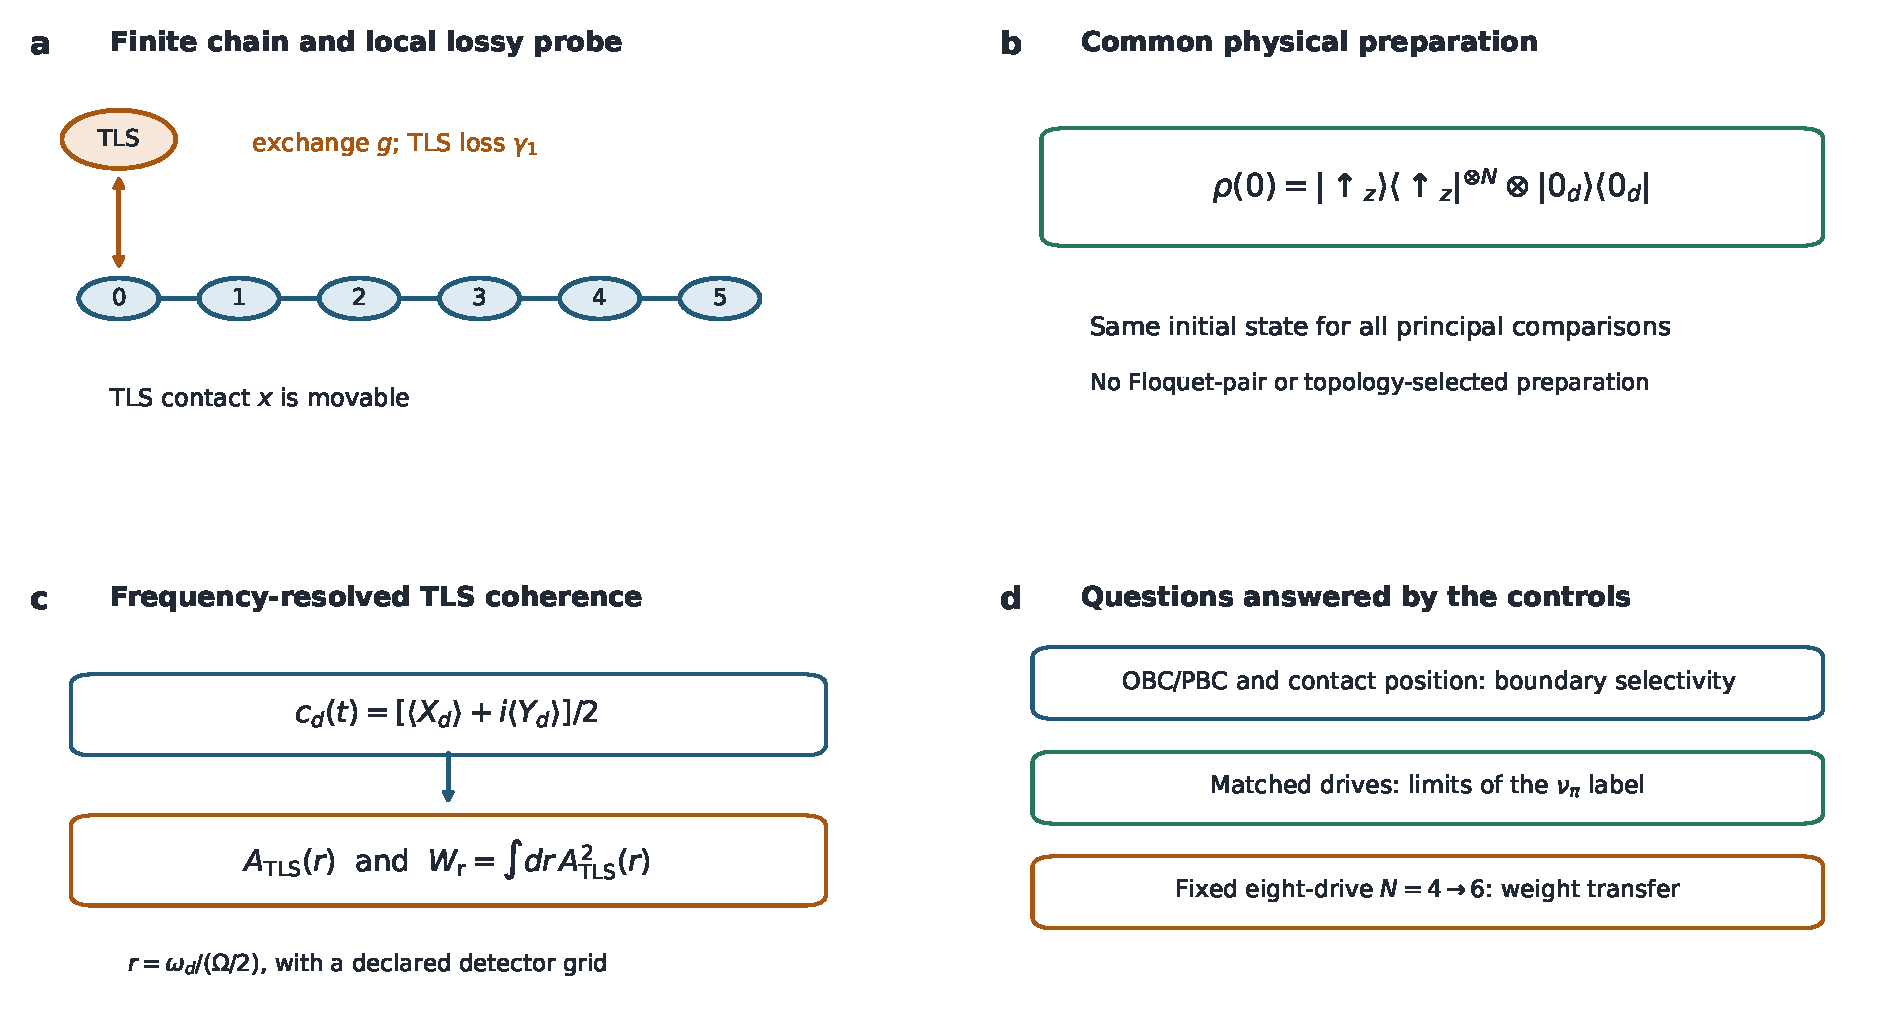
\includegraphics[width=\textwidth]{fig1_model_common_preparation_workflow.pdf}
\caption{Local probe and controlled readout. (a) A two-step Ising chain is coupled at contact $x$ to an amplitude-damped TLS. (b) The same product preparation is used for each principal full-model comparison. (c) Varying the TLS splitting produces a frequency-resolved coherence and its raw integrated weight. (d) Contact, boundary condition, and matched-drive controls test which features of the signal are specific to the open-chain boundary. Closed-chain BDI labels organize drives; they do not set the dissipative initial state.}
\label{fig:workflow}
\end{figure}

\section{Common product preparation and spectroscopy observables}
\label{sec:observables}

Every principal full-model comparison begins from
\begin{equation}
\begin{aligned}
\rho(0)&=\left(\ket{\uparrow_z}\bra{\uparrow_z}\right)^{\otimes N}
\otimes\ket{0_d}\bra{0_d},\\[-2pt]
N&=6.
\end{aligned}
\label{eq:common-preparation}
\end{equation}
This declaration rules out Floquet-pair, numerical-mode, and topology-dependent preparation selection.

The TLS detector ratio is $r=\omega_d/(\Omega/2)$, where $\Omega=2\pi/T$. The transverse TLS coherence is $c_d(t)=[\expect{X_d(t)}+\ii\expect{Y_d(t)}]/2$. Define the retained-window mean $\overline{c_d}=(t_f-t_{\rm dis})^{-1}\int_{t_{\rm dis}}^{t_f}\dd t\,c_d(t)$. The baseline-subtracted complex subharmonic phasor is
\begin{equation}
\begin{aligned}
\widetilde A_{\rm TLS}(r)&=\frac{2}{t_f-t_{\rm dis}}\int_{t_{\rm dis}}^{t_f}\!\dd t\,
[c_d(t)-\overline{c_d}]e^{\ii\Omega t/2},\\
A_{\rm TLS}(r)&=|\widetilde A_{\rm TLS}(r)|.
\end{aligned}
\label{eq:phasor}
\end{equation}
The raw integrated response is $\Wraw=\int\dd r\,A_{\rm TLS}^2(r)$. The principal detector grid is $r_q=0.880+0.024q$ for $q=0,\ldots,10$. For shape comparisons we use the normalized distance $D(a,b)=\lVert a/\lVert a\rVert_2-b/\lVert b\rVert_2\rVert_2$. For the damping scan, the same baseline-subtracted transform applied to $\expect{Z_0(t)}$ defines the edge phasor $\widetilde A_{\rm edge}$ and $A_{\rm edge}=|\widetilde A_{\rm edge}|$. Its stroboscopic subharmonic component is
\begin{equation}
M_{\pi,{\rm edge}}=\left|\frac{1}{N_{\rm ret}}\sum_{n\in{\rm retained}}(-1)^n\expect{Z_0(nT)}\right|,
\end{equation}
and the reported TLS emission proxy is $P_{\rm em}=\gamma_1\overline{\expect{n_d}}$, with the mean taken over the retained continuous-time samples. A relative phase is obtained from the relevant complex phasors and is reported only where both amplitudes exceed a finite visibility threshold; a phase at vanishing response is not interpreted.

\section{Boundary-selective exact full-model response}
\label{sec:boundary-response}

\Cref{fig:boundary} tests geometry without tailoring the preparation to a particular Floquet mode. At the held-out drive, changing only the chain boundary condition reduces the integrated TLS response from $W_{\mathrm r}^{\mathrm{OBC}}=2.5261\times10^{-3}$ to $W_{\mathrm r}^{\mathrm{PBC}}=2.6486\times10^{-7}$, a directional OBC/PBC ratio of $9.54\times10^3$. Independently, moving the TLS along the open chain gives $\Wraw(0)=3.3247\times10^{-3}$, $\Wraw(1)=6.3759\times10^{-4}$, and $\Wraw(3)=3.3875\times10^{-6}$: the edge exceeds its neighbor by $5.214$ and this interior contact by $9.81\times10^2$. These ratios use the stored nonzero denominators without a floor. Together, the boundary-condition and position changes establish a strong finite-system boundary contrast in the local readout. They do not, by themselves, identify the microscopic source of the signal as topological. Sampling and retained-window checks are detailed in the Supplemental Material.

\begin{figure}[t]
\centering
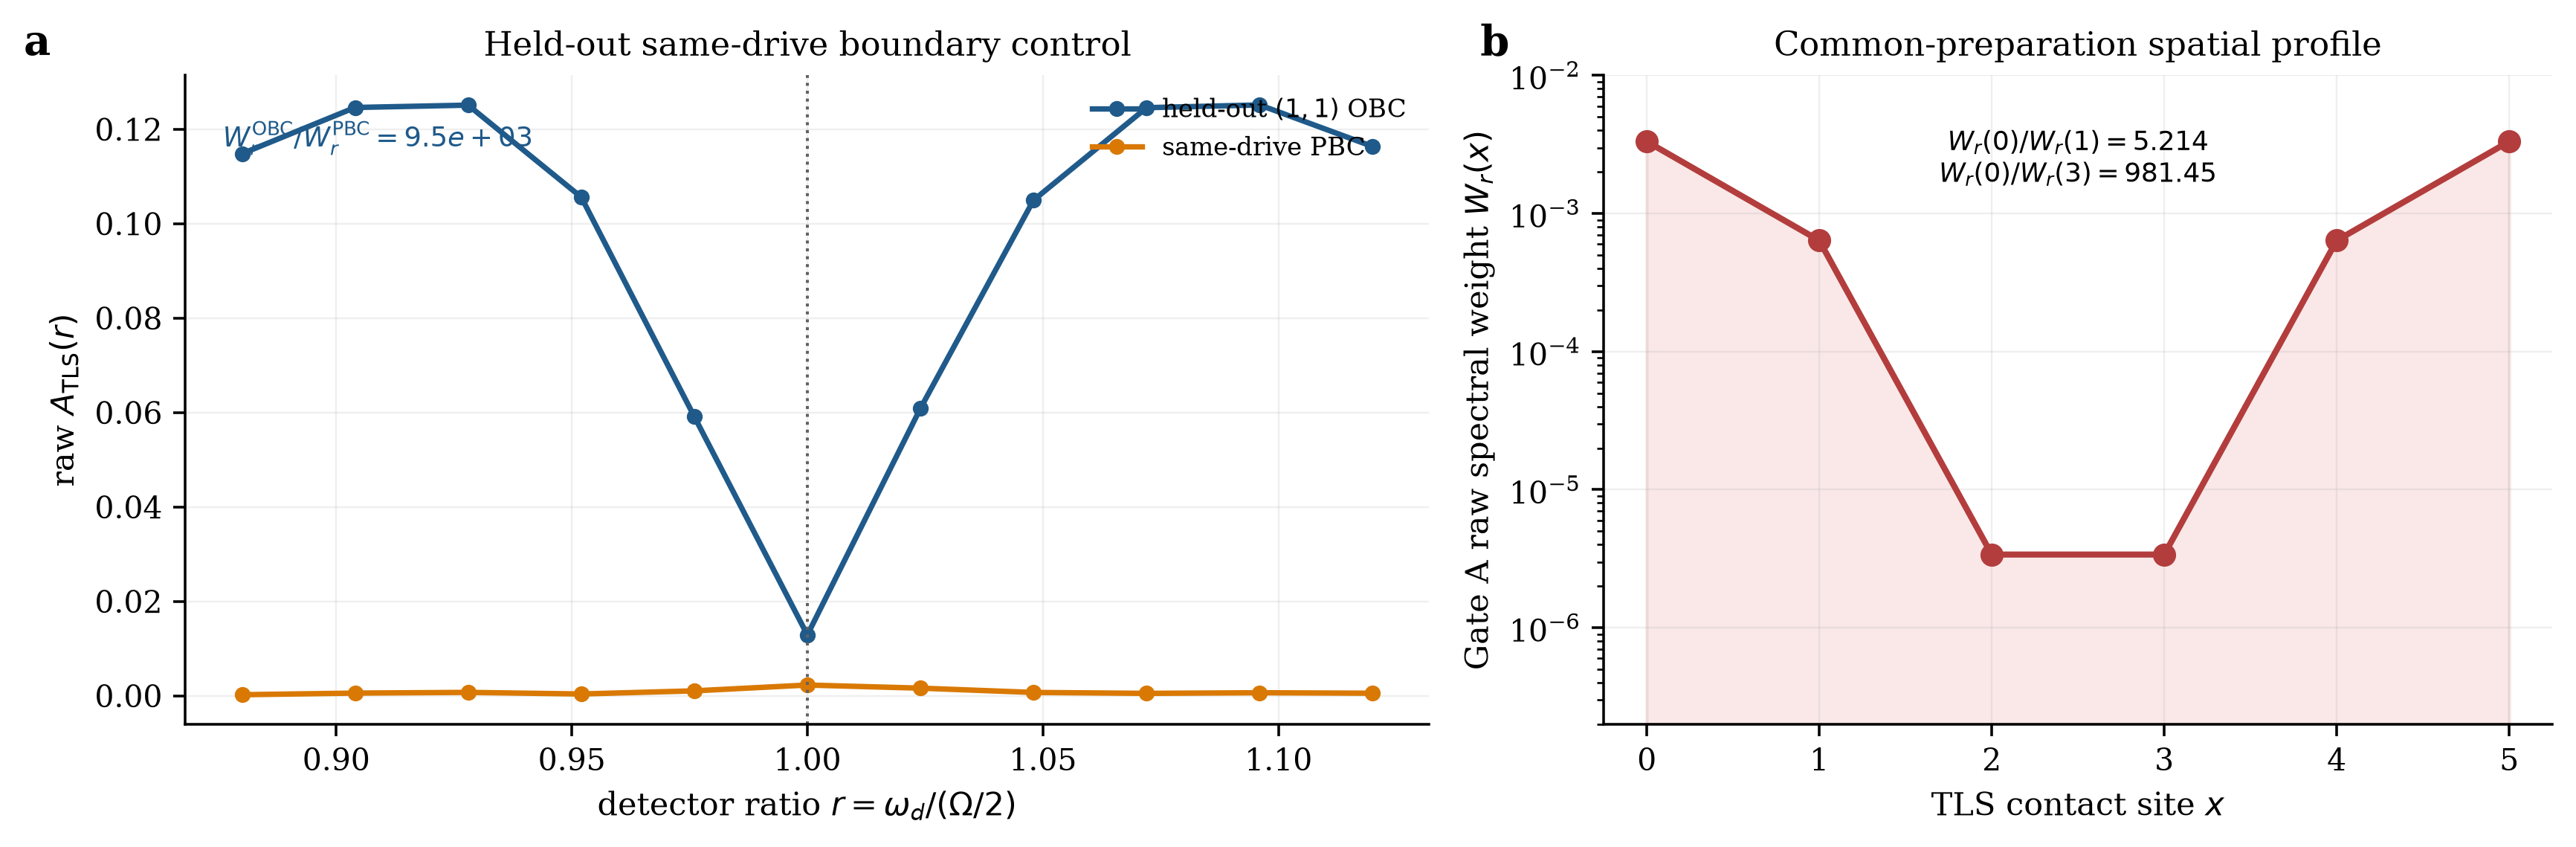
\includegraphics[width=\textwidth]{fig2_boundary_geometry_response.png}
\caption{Geometry dependence of the full-model TLS response at $N=6$. (a) The same-drive open-chain and periodic-chain spectra, with raw integrated weights in the declared OBC/PBC order. (b) The spectral weight for contacts $x=0,\ldots,5$ under the same product preparation. The observed contrast is a finite-chain readout; no localization length or thermodynamic invariant is extracted.}
\label{fig:boundary}
\end{figure}

\FloatBarrier

\section{Matched controls and limits of the topological interpretation}
\label{sec:bdi-controls}

The geometry contrast motivates asking whether a closed-chain BDI label predicts the measured spectrum. We compare two same-period drive pairs: $(1,1)$ versus $(0,1)$ at $T=2.591813939212$, and $(1,0)$ versus $(0,0)$ at $T=1.295906969606$. Each pair changes $\nu_0$ at fixed $\nu_\pi$. The four drives do not form a single common-period four-class experiment; the comparison tests the response within each matched line and checks for an empirical grouping across the sampled spectra. Numerical settings and window checks are in the Supplemental Material.

\Cref{fig:matched-controls} shows that drives sharing $\nu_\pi$ can still produce distinct normalized responses: their within-label shape distances are $0.6865$ and $0.4661$. Cross-label distances range from $0.1532$ to $0.7114$, overlapping the within-label values. Thus the tested spectra do not group by $\nu_\pi$ alone. This observation constrains a label-only interpretation of local TLS spectroscopy without claiming that these four drives isolate a causal effect of $\nu_\pi$ at one common period.

\begin{figure}[t]
\centering
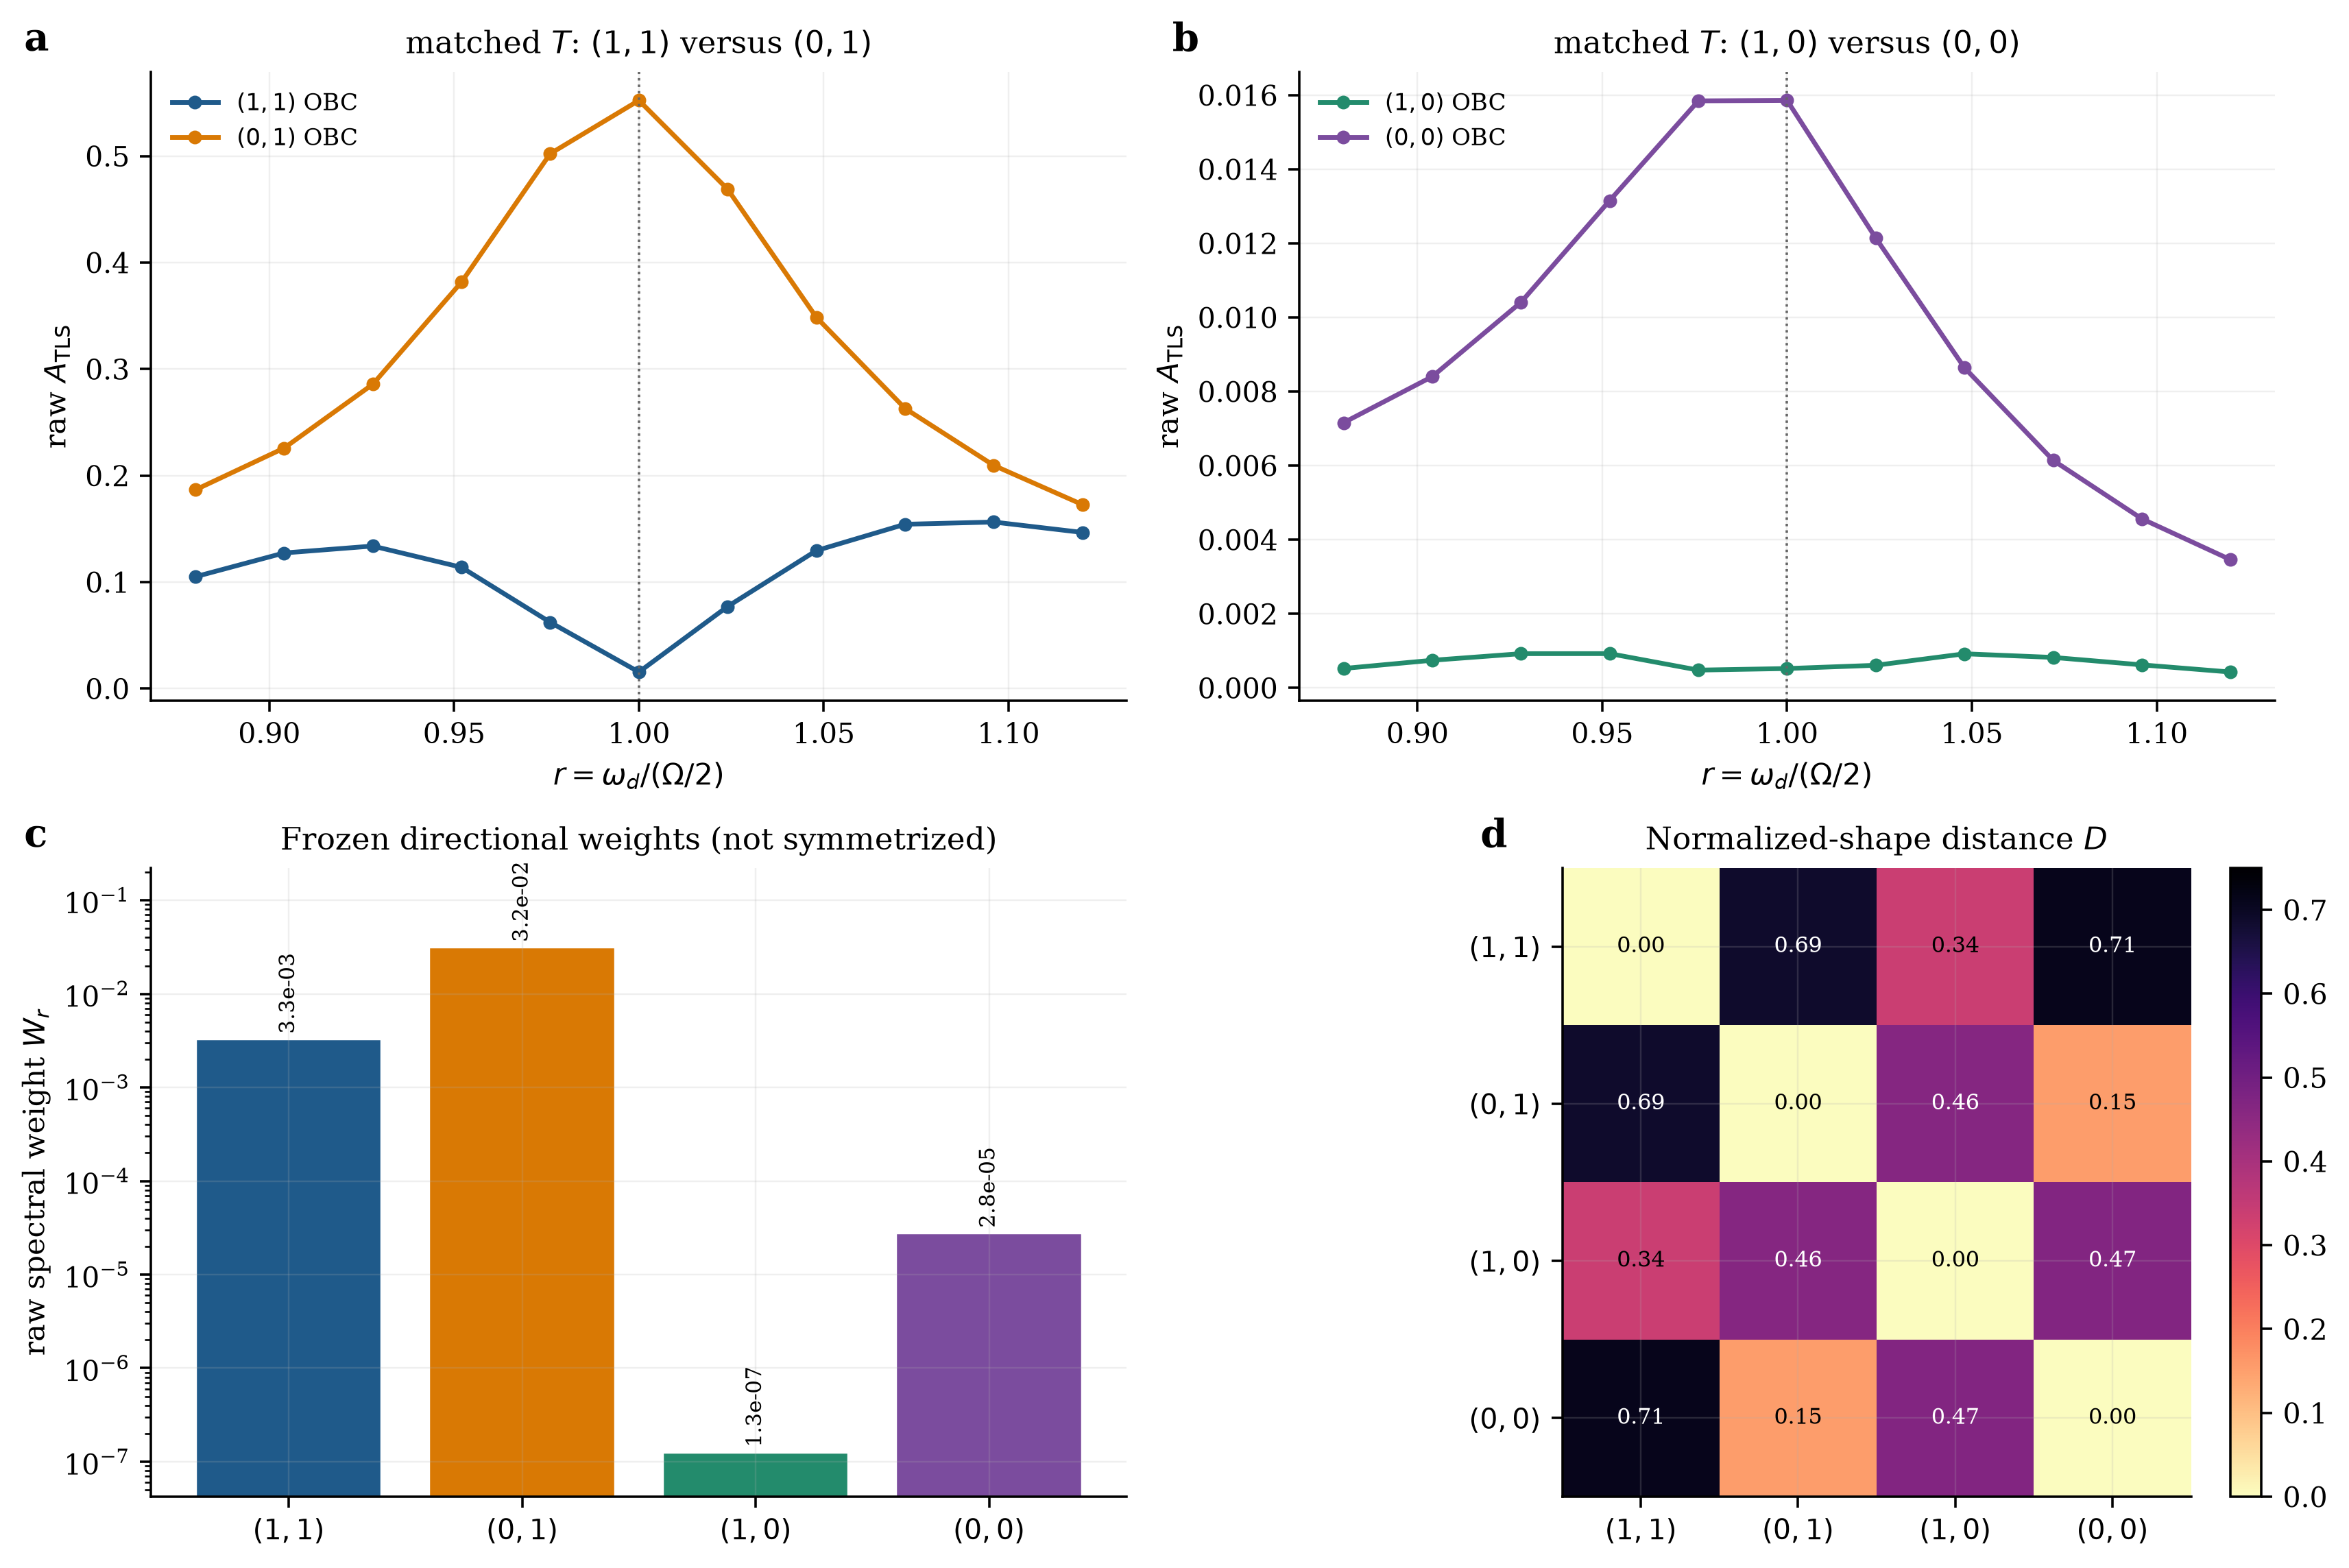
\includegraphics[width=\textwidth]{fig3_matched_controls_shape_distance.png}
\caption{Drive dependence of the local spectrum. (a,b) TLS spectra and directional integrated weights for two same-period pairs, $(1,1)$ versus $(0,1)$ and $(1,0)$ versus $(0,0)$. (c) Pairwise distances between normalized spectra. Within- and cross-$\nu_\pi$ distances overlap in this four-drive sample.}
\label{fig:matched-controls}
\end{figure}

\FloatBarrier

\section{Finite-size transfer of the response-weight hierarchy}
\label{sec:gate-d2}

The preceding shape test and a size-transfer test address distinct questions. We ask whether the ordering of raw integrated weights observed in an eight-drive $N=4$ table survives when the same drives and detector grids are evaluated at $N=6$. The drives and three pass conditions were specified before inspecting the $N=6$ results; all eight points are retained. The exact tasks, thresholds, and validation record are given in the Supplemental Material.

\begin{figure}[t]
\centering
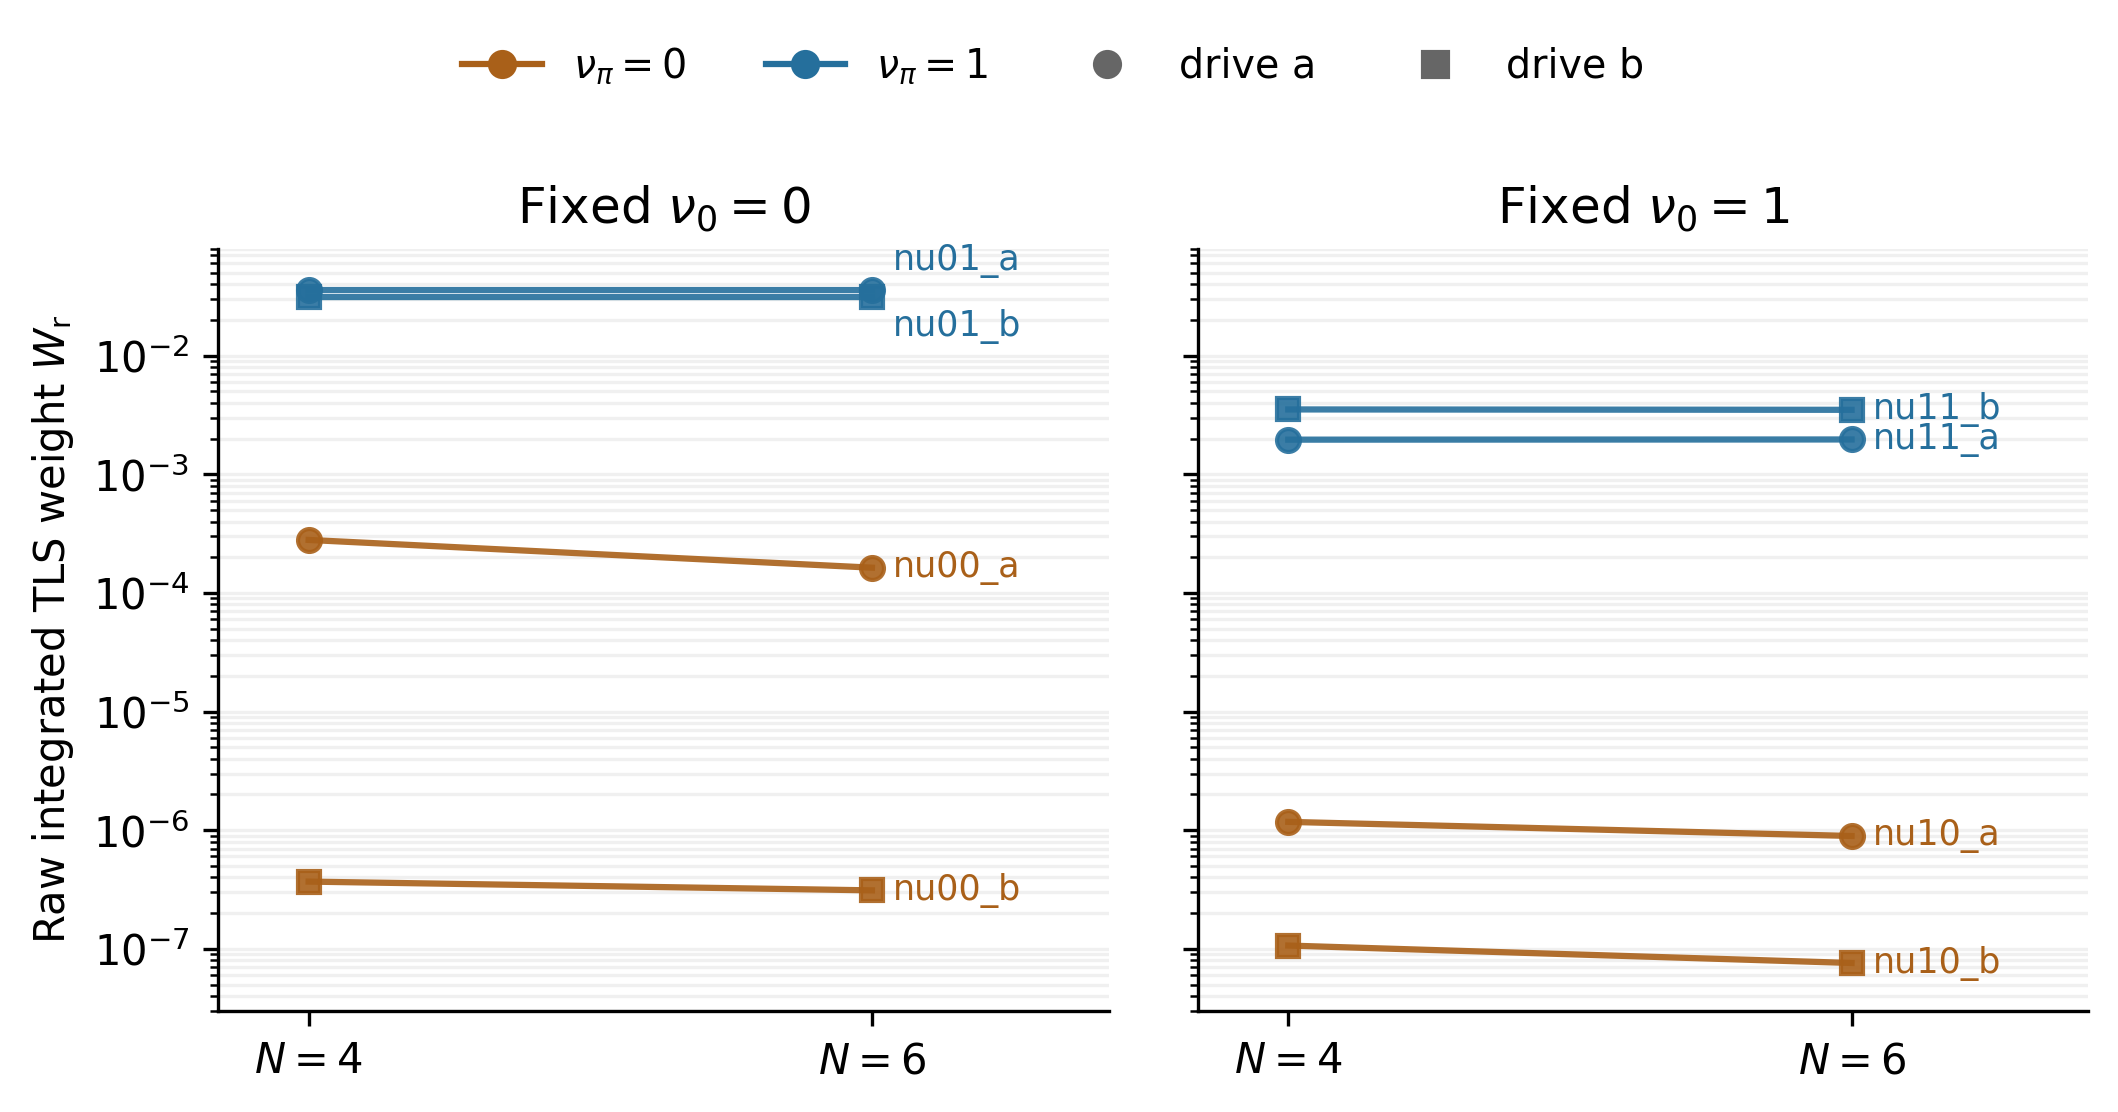
\includegraphics[width=\textwidth]{fig4_d2_weight_transfer.png}
\caption{Eight predefined drives followed from $N=4$ to $N=6$. Each line joins the same drive ID at two sizes; color denotes its closed-chain $\nu_\pi$ label, and marker shape distinguishes the two drives in each class. Both panels use a common logarithmic raw-weight axis. Within fixed $\nu_0=0$ and $1$, the $N=6$ ratios of the $\nu_\pi=1$ to $\nu_\pi=0$ class medians are $409.54$ and $5633.72$. The minimum $\nu_\pi=1$ weight exceeds the maximum $\nu_\pi=0$ weight by $12.05$. The $\nu_\pi$ strata have different drive periods; lines connect sizes, not matched causal contrasts between labels.}
\label{fig:d2-transfer}
\end{figure}

\Cref{fig:d2-transfer} shows that the frozen raw-weight ordering passes at $N=6$. At fixed $\nu_0=0$ and $1$, the ratios of the $\nu_\pi=1$ to $\nu_\pi=0$ class medians are $409.54$ and $5633.72$ (threshold $>10$); the minimum $\nu_\pi=1$ weight divided by the maximum $\nu_\pi=0$ weight is $12.05$ (threshold $>1$). This is evidence that the sampled weight hierarchy persists across the two finite sizes. Because the two label strata include different periods, it is not a same-period causal test of $\nu_\pi$. Raw weight can retain a hierarchy even when normalized line shapes fail to group by that label; neither result is a thermodynamic invariant.

\FloatBarrier

\section{TLS hybridization and dissipative backaction}
\label{sec:hybridization-backaction}

\subsection{Coupling-resolved response doublets}

The TLS is not merely a readout channel: changing its exchange coupling changes the spectrum. In the four internally resolved spectra at $g/J=0.06$--$0.12$, the TLS response develops a coupling-dependent doublet near detector ratio one [\cref{fig:tls-spectroscopy}]. A free-intercept fit over this finite interval gives $\Delta\omega/J=3.4527(g/J)-0.07333$ and $R^2=0.9982$. Its nonzero intercept and the unresolved weaker-coupling points prevent extrapolation to a zero-coupling law. At fixed contact and harmonic, $g_{\rm eff}=g|B_{0\pi}(0,0)|$ is a constant rescaling of $g$, so this fit alone does not test the absolute projected matrix element. The alternative origin-constrained fit, residuals, and window dependence are reported in the Supplemental Material.

\begin{figure}[t]
\centering
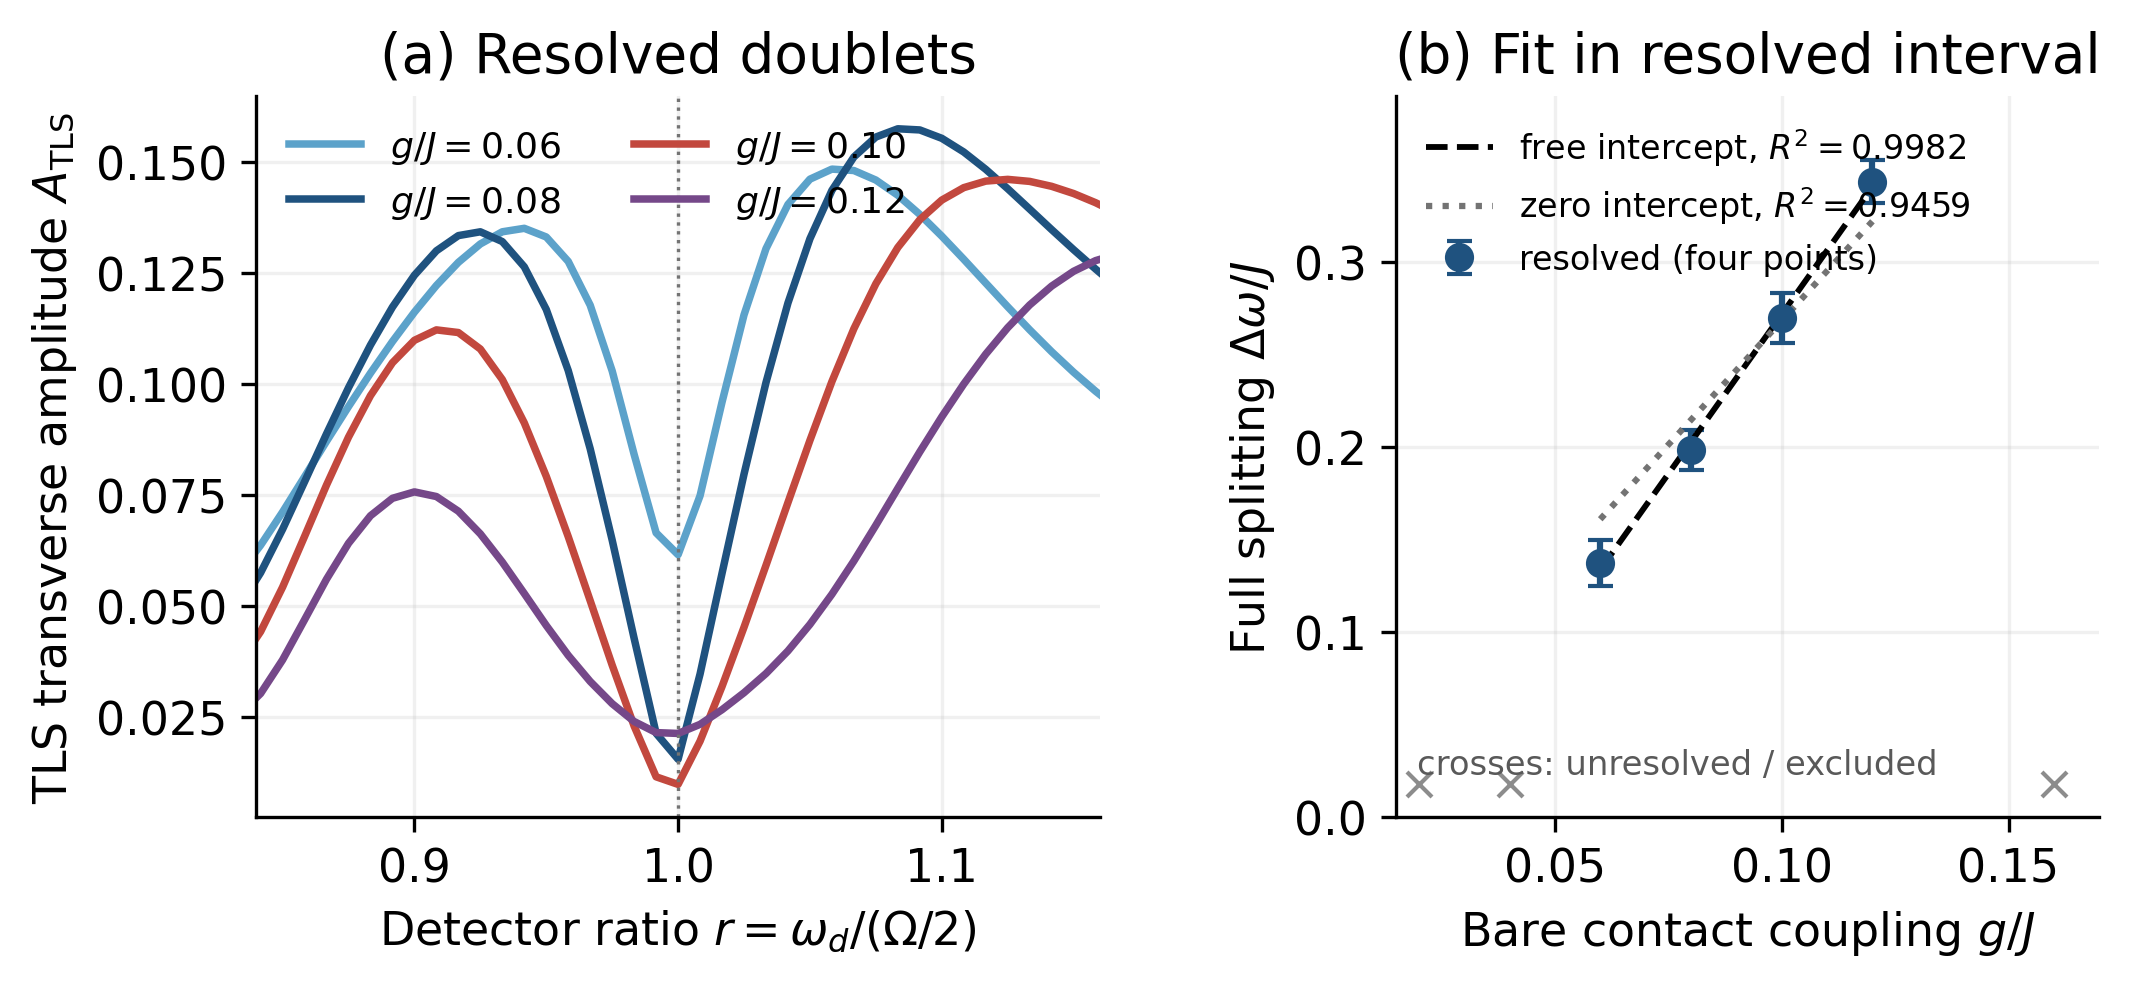
\includegraphics[width=\textwidth]{fig3_theory_tested_tls_spectroscopy.png}
\caption{Coupling-resolved Floquet--TLS response. (a) Four representative $N=6$ transverse TLS spectra show coupling-dependent response doublets. (b) The full splitting against bare $g/J$ for four internally resolved points, with free-intercept and origin-constrained lines shown only over that interval. Vertical bars show the deterministic standard deviation across the $8T$, $20T$, and $40T$ discard-window extractions; they are not statistical error bars. Crosses placed near the baseline identify unresolved or excluded scan settings and do not encode a measured zero splitting. The detuning-dependent edge/TLS amplitudes and visibility-masked relative phase are shown in the Supplemental Material.}
\label{fig:tls-spectroscopy}
\end{figure}

\subsection{Loading followed by fast-loss recovery}

Varying only the TLS relaxation rate gives a nonmonotonic boundary response. At $N=6$, $g/J=0.08$, and detector ratio one, the edge amplitude and alternating stroboscopic edge component are most strongly suppressed near $\gamma_1T\simeq0.317$. At larger rates the TLS transverse amplitude decreases while the edge signal recovers, reaching $A_{\rm edge}=0.641$ and $M_{\pi,\rm edge}=0.541$ at $\gamma_1T\simeq7.775$. These values come from 31 completed rates over 80 periods with a $20T$ discard; the emission proxy reaches a broad maximum at weaker damping [\cref{fig:damping-backaction}].

For interpretation, eliminating a rapidly relaxing TLS gives the induced edge-decay scale
\begin{equation}
\Gamma_{\rm TLS}(\Delta_\ell)=\frac{4|g_{x,\ell}|^2\gamma_1}{\gamma_1^2+4\Delta_\ell^2},
\label{eq:induced-decay}
\end{equation}
which decreases as $4|g_{x,\ell}|^2/\gamma_1$ on resonance at large $\gamma_1$.

\FloatBarrier
\begin{figure}[t]
\centering
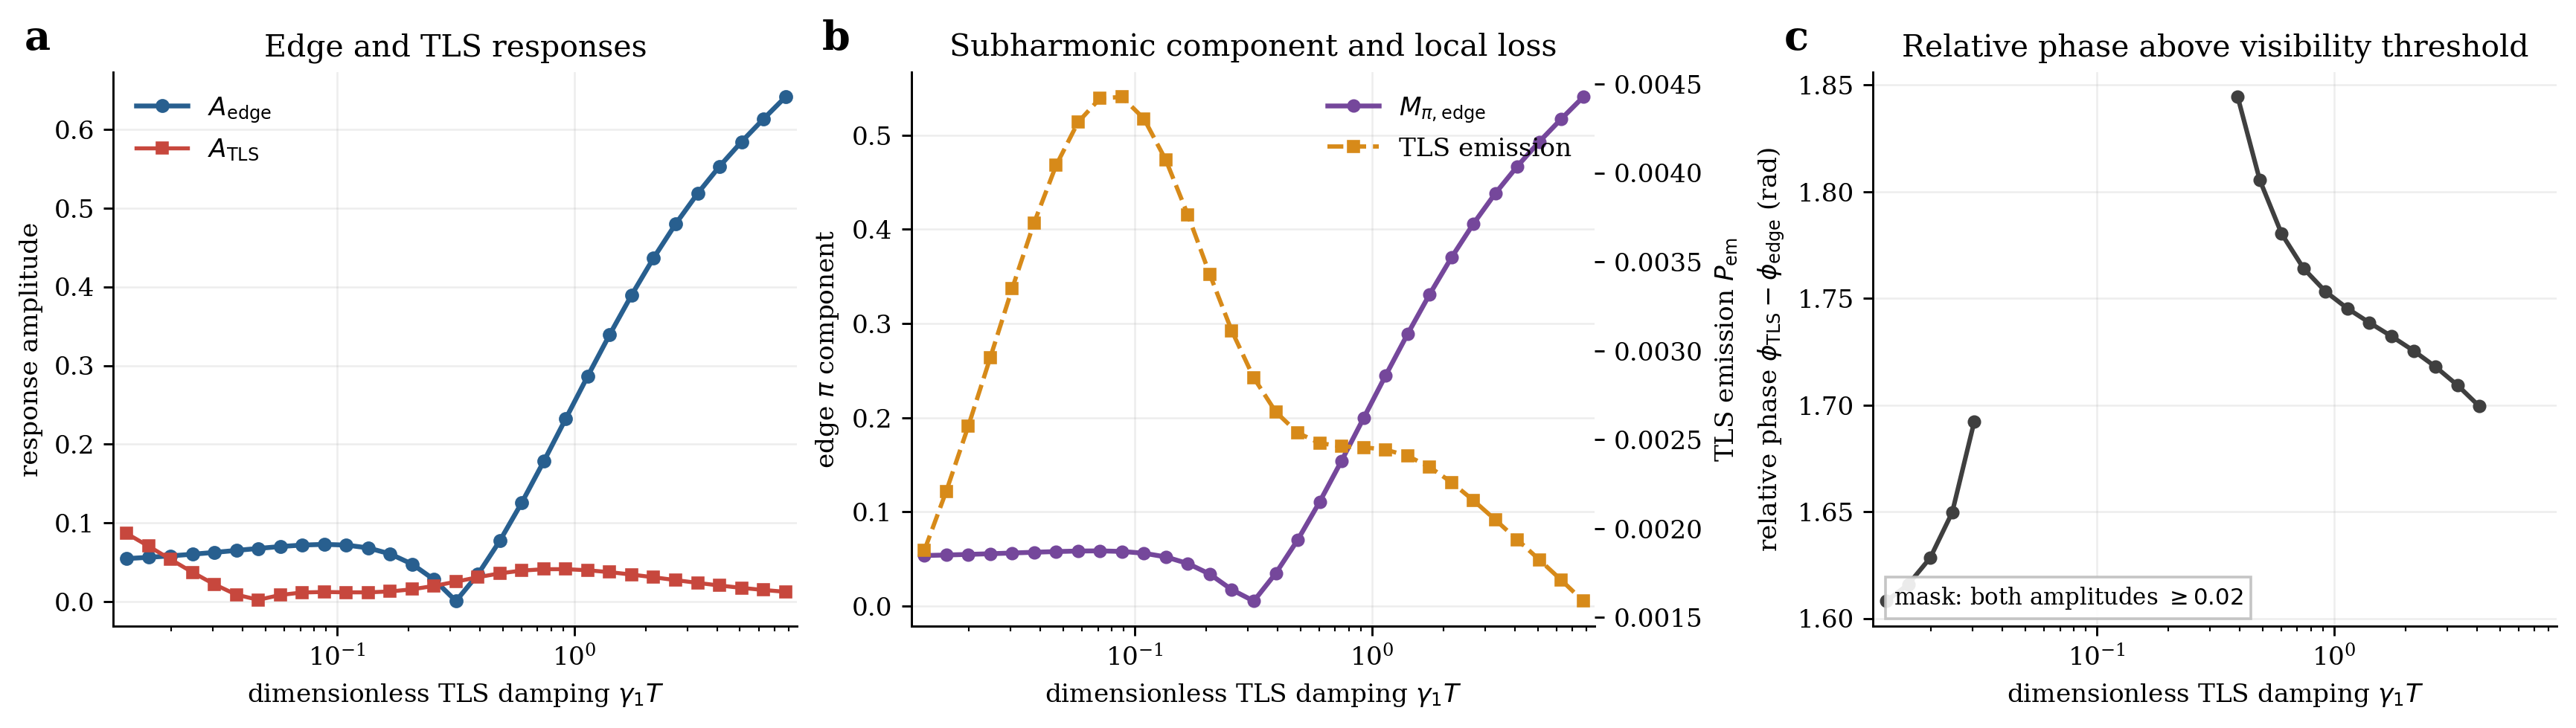
\includegraphics[width=\textwidth]{fig5_dissipation_backaction_gammaT.png}
\caption{Dissipation-controlled backaction at fixed $N=6$, $g/J=0.08$, detector ratio one, and 80 Floquet periods. The horizontal axis is the dimensionless rate $\gamma_1T$. (a) Edge and transverse TLS response amplitudes. (b) Stroboscopic edge $\pi$ component and $P_{\rm em}=\gamma_1\overline{\expect{n_d}}$. (c) Relative phase only where both complex phasors exceed the stated visibility threshold. The suppression followed by recovery is consistent with fast-defect elimination or Zeno-like decoupling; no fitted transition or independently defined regime boundary is claimed.}
\label{fig:damping-backaction}
\end{figure}

The falloff in \cref{eq:induced-decay} is consistent with the observed recovery under rapid relaxation. This fast-defect or Zeno-like interpretation has not been quantitatively fitted to the full response; the finite-rate crossovers are not phase transitions. Together with the doublet, the scan shows that the probe changes the very boundary dynamics whose spectrum it records.

\FloatBarrier

\section{Reduced multichannel diagnostics and limitations}
\label{sec:limitations}

A projection onto edge-related Floquet channels offers a physical language for local sidebands and hybridization, provided its range of validity is checked. The exact $N=4$ channel/time benchmark compares one conjugate channel pair with an independently initialized late-time fit. At $N=6$, the available evidence consists of edge-seeded, residual-qualified conjugate Ritz pairs near $-1$ with nonzero edge visibility; it does not give the exhaustive spectrum or a channel/time lifetime-equality test.

The $K$-channel and $N=6$/$N=8$ comparisons test a different, Floquet-pair-prepared representation and cannot independently validate the common-product full-model response. In a more direct spatial stress test, matching one edge dressed scale required bare couplings $g=0.08$, $1.60461$, and $27.0097$ at $x=0$, $1$, and $2$; the interior spectra then failed to retain a stable near-resonant doublet across the checked windows. The projected picture is consequently useful near the resolved edge-contact regime but does not yield a contact-independent multichannel collapse. Channel benchmarks, truncation audits, and the failed continuation appear in the Supplemental Material.

\section{Discussion and conclusion}
\label{sec:discussion}

The central result is a geometry-dependent local observable of a finite driven open system. With the same product preparation, the TLS sees a strong open-boundary response that weakens at interior contacts and in the periodic chain. This is a useful operational distinction: a probe can reveal a boundary without its signal being a direct meter of the closed-chain invariant. Indeed, the tested normalized spectra depend on the drive within a fixed $\nu_\pi$ class. The frozen eight-drive comparison does establish that a separate raw-weight hierarchy persists from $N=4$ to $N=6$, but its periods differ across the label strata. The two results can coexist because spectral shape and integrated power are different observables.

The probe's influence is part of that interpretation. Its coupling produces a resolved doublet over a finite interval, and intermediate loss suppresses the edge response before rapid loss allows recovery. A projected edge--TLS model rationalizes these trends but fails as a general description of the prepared full response across all contacts and couplings. The calculation thus identifies a finite, drive-dependent readout and an active source of backaction. It does not establish a universal $\pi$-edge spectroscopy, a thermodynamic invariant, or a persistent time-crystalline phase. A larger common-period drive ensemble, controlled size scaling, and a platform-specific bath model would be needed to test those broader possibilities.

\section*{Supplemental Material}

See Supplemental Material for the detailed analysis contract, numerical-window checks, complete coupling and damping scans, the channel/time benchmark, the reduced-model failure tests, and the fixed eight-drive transfer table. Provenance and reproduction commands are included there; immutable task records are maintained in the versioned repository.

\section*{Data availability}
The versioned protocols, numerical checkpoints, result records, figure generators, and read-only audits are available in the \href{https://github.com/666888rwy-bit/floquet-tls-pi-edge-tls}{public GitHub repository}. The frozen $N=6$ transfer records and their manifest were committed separately from the source freeze (result commit \texttt{a3d9dc3}); the figure sources are on the \href{https://github.com/666888rwy-bit/floquet-tls-pi-edge-tls/tree/manuscript-pra-regular-article}{PRA manuscript branch}. An archival DOI specific to these results has not yet been assigned.

\section*{Code availability}
The exact sparse Floquet--Lindblad propagation, deterministic figure generators, channel analyses, and submission checks are available under the MIT License in the repository listed above.

\section*{Acknowledgments}
OpenAI ChatGPT (Codex, GPT-6) assisted with restructuring and drafting parts of the manuscript under the author's stated scientific claim boundaries. Numerical claims were checked against versioned result records, and the newly added references against publisher records. The author remains responsible for independently reviewing the final text, references, and interpretation before submission.

\bibliographystyle{unsrtnat}
\bibliography{references}

\end{document}
